\section{Extended studies}\label{sec:studies}
The results of Section~\ref{sec:results} rest on several fixed choices: a \SI{5}{K} cooler pinch, no pressure drops, one price per kilogram, an undiscounted payout, a single design point, \SI{500}{\celsius} at the turbine and \SI{20}{MPa} at its inlet. After the submission we tested each of these in nine separate studies. Each study varies one thing and re-ranks, under both the main and the strict reading of the \SI{7.7}{MPa} limit. Table~\ref{tab:studies} summarises them; the paragraphs below give the details.

The designs followed through the studies are:
\begin{itemize}
  \item \textbf{Selected} (main TOPSIS first): layout 6, \SI{33.5}{\celsius}, $\Pm = \SI{7.9}{MPa}$, $\Pe = \SI{3.7}{MPa}$, $x = 0.38$;
  \item \textbf{Strict winner} (strict TOPSIS first): layout 3, \SI{32.5}{\celsius}, $x = 0.46$; and the strict knee, layout 3, \SI{33}{\celsius}, $x = 0.43$;
  \item \textbf{Highest payout}: layout 3, \SI{32}{\celsius}, $x = 0.36$;
  \item \textbf{Submitted}: layout 3, \SI{33}{\celsius}, $x = 0.40$, the design recommended in the submitted report;
  \item \textbf{Reference}: the recuperated reference.
\end{itemize}

\begin{table}[h]\centering\footnotesize
\setlength{\tabcolsep}{4pt}
\begin{tabularx}{\textwidth}{@{}l >{\raggedright\arraybackslash}X >{\raggedright\arraybackslash}X >{\raggedright\arraybackslash}X@{}}
\toprule
Study & What was varied & Main ranking (ours) & Strict ranking\\
\midrule
S1 & Cooler pinch 3 and \SI{8}{K}, all designs re-solved & Holds at \SI{8}{K}; at \SI{3}{K} moves to layout 3 ($x = 0.47$) & Holds (layout 3, \SI{32.5}{} to \SI{33}{\celsius})\\
S2 & Compressor inlet 32 to \SI{36}{\celsius}, recuperators frozen & Selected design loses 0.25 points/K & Winner loses 1.2 points/K\\
S3 & Pressure drop 1\% and 2\% per exchanger side, all designs re-solved, $M_0$ fixed & Holds; TOPSIS first unchanged & Holds (layout 3, \SI{32.5}{\celsius}, $x$ = 0.45 to 0.46)\\
S4 & Exchanger and machinery priced separately & Holds up to a price ratio of 2; layout 3 at 4 and above & Holds\\
S5 & Discounting, 0 to 10\%, $N$ = 10 and 20 & Holds & Holds\\
S6 & Turbine inlet 400 to \SI{500}{\celsius} & Valid throughout; gains most from high temperature & Valid throughout\\
S7 & $\Ph$ 14 to \SI{20}{MPa} & \SI{20}{MPa} remains best & \SI{20}{MPa} remains best\\
S8 & Layout 1 with cooling water at up to 100 bar & No change & No change\\
S9 & Temperature profiles of every exchanger & Diagnostic & Diagnostic\\
\bottomrule
\end{tabularx}
\caption{The extended studies and whether each recommendation holds.}\label{tab:studies}
\end{table}

\paragraph{S1: cooler pinch.} All 2656 designs were re-solved with a cooler pinch of \SI{3}{K} and of \SI{8}{K}, and $M_0$ was recalibrated each time (the reference stays the same design; $M_0$ becomes \SI{31.6}{t} at \SI{3}{K} and \SI{45.0}{t} at \SI{8}{K}). The pinch changes only the coolers and the water flow, not the cycle. At \SI{8}{K} every design with a compressor inlet of 32 or \SI{32.5}{\celsius} becomes impossible: the water enters at \SI{25}{\celsius}, so the cold end of the cooler can offer at most 7 or \SI{7.5}{K}. These 569 designs, including the strict winner and the highest-payout design, are removed; the main ranking still selects layout 6 (at \SI{33}{\celsius}, $\Pe = \SI{4.5}{MPa}$, $x = 0.30$), and the strict ranking moves to layout 3 at \SI{33}{\celsius}. The \SI{8}{K} pinch also multiplies the water flow of the remaining winners several times. At \SI{3}{K} the coolers grow by about \SI{7}{t}; the main ranking then tips to recompression ($x = 0.47$), which shows how close the two layouts are.

\paragraph{S2: compressor inlet drift.} This is the closest the model comes to off-design behaviour. For each design the recuperators were frozen at their design conductance, the pressures and split were held, and the compressor inlet temperature was moved from 32 to \SI{36}{\celsius} (Figure~\ref{fig:s2}). The coolers could not be frozen, because the solver's cooler accepts only a pinch specification, so they keep the \SI{5}{K} pinch. The frozen model reproduces every design point to within $2\times10^{-5}$ in efficiency. The recompression designs lose 1.0 to 1.4 points of efficiency per kelvin, most of it between 32.5 and \SI{33.5}{\celsius}, where their \SI{7.7}{MPa} inlet crosses the pseudo-critical line and its density falls from about 550 to \SI{365}{kg/m^3}. The selected partial-cooling design is almost flat up to \SI{34}{\celsius} and loses only 0.25 points per kelvin over the range; above \SI{33.75}{\celsius} it is more efficient than the submitted recompression design. Where the inlet temperature cannot be held tightly, this favours the selected design. The test keeps the machine efficiencies, pressures and split fixed and uses no compressor or turbine maps, so the rates are those of the cycle at fixed hardware, not of a controlled plant; the difference between the two layouts, a factor of four to six, is the result we rely on.

\begin{figure}[h]\centering
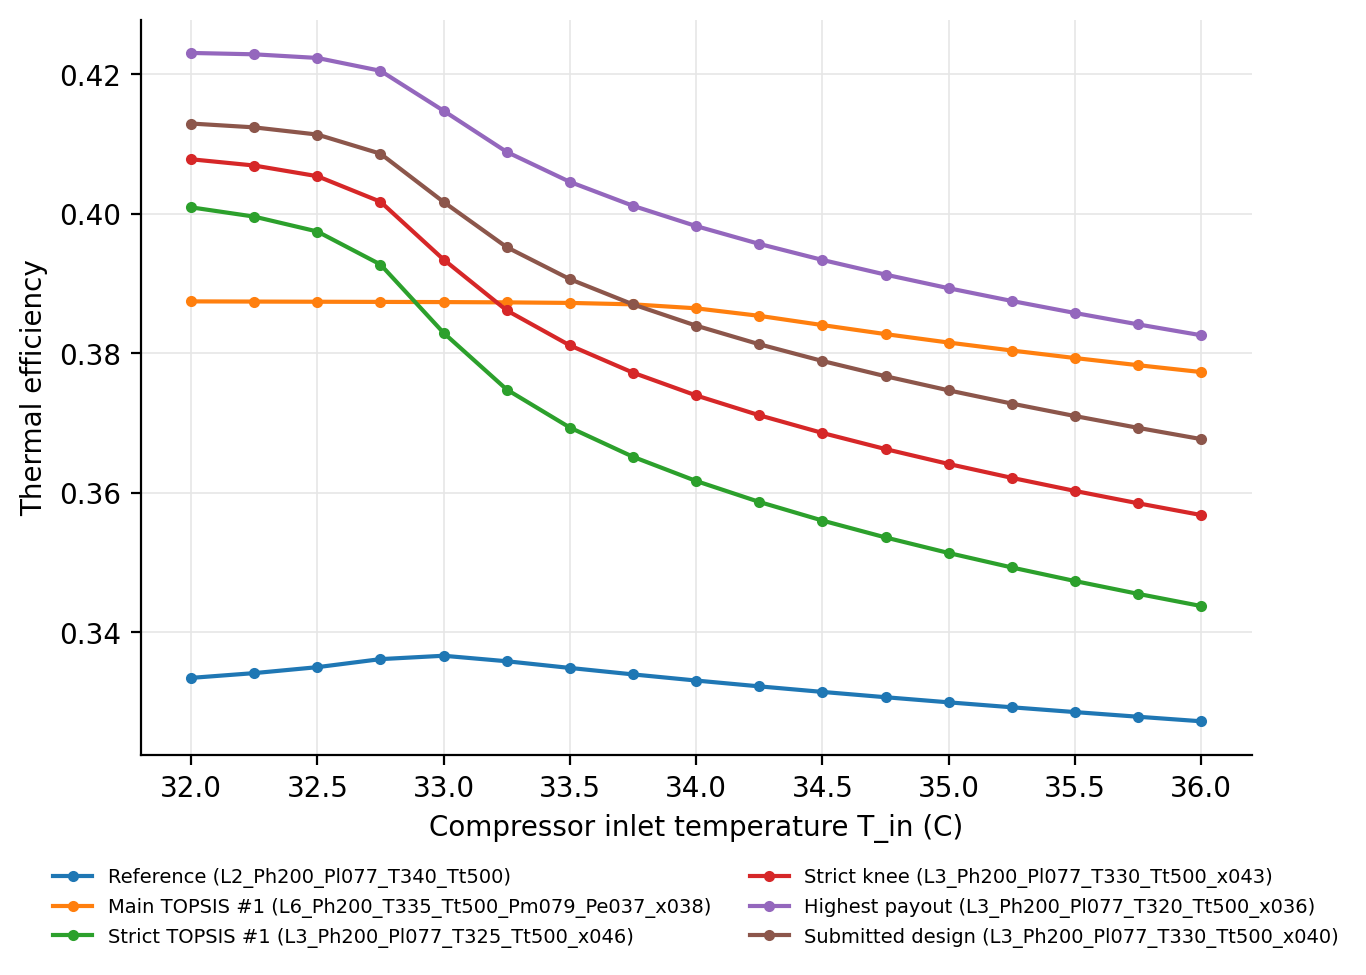
\includegraphics[width=0.8\textwidth]{figs/s2_drift.png}
\caption{S2: efficiency against compressor inlet temperature with the recuperators frozen at their design size.}\label{fig:s2}
\end{figure}

\paragraph{S3: pressure drops.} All designs were re-solved with a pressure loss of 1\% and then 2\% of inlet pressure on both sides of every recuperator, every cooler and the heater. The best efficiency of each layout falls by 1.0 to 1.7 points at 1\% and by 2.1 to 3.6 points at 2\%. The recompression layouts lose most (layouts 3 and 5, 1.7 points at 1\%), partial cooling less (1.4) and the recuperated layouts least (1.0). $M_0$ is held at its baseline value of \SI{39.06}{t}. Recalibrating it would make a heavier recuperated design at \SI{9.7}{MPa} the most efficient of layout~2 and drop $M_0$ to about \SI{20}{t}; that shifts every mass by the same constant, which leaves the Pareto front and the knee unchanged but distorts TOPSIS, which scales each objective by its vector length.

With $M_0$ fixed, the selected design remains first by TOPSIS in the main ranking at both levels, and the knee moves only in $\Pe$ (to 3.8 and \SI{3.7}{MPa}). The strict ranking stays with layout~3 at \SI{32.5}{\celsius} ($x = 0.46$ at 1\%, 0.45 at 2\%), and its knee becomes the same design. Pressure drops favour the selected design: it loses 1.5 points at 1\% and 3.0 points at 2\%, against 1.8 and 3.9 for the strict winner. At 2\% its payout (\$157.4M) is within \$0.2M of the strict winner's (\$157.5M) at \SI{3.8}{t} less mass, and its incremental payback against the reference at the same pressure drop (0.93 years) is shorter than that of every named recompression design (1.27 to 1.39 years). Pressure drops were applied to designs optimised without them; the designs were not re-optimised with losses included.

\paragraph{S4: separate prices.} Exchanger mass was priced at $c_\mathrm{hx}$ and all other mass at $c_\mathrm{tm}$, with $c_\mathrm{tm}/c_\mathrm{hx}$ = 0.5, 1, 2, 4 and 8, keeping the reference design at \$15M in every case. The main ranking stays with layout 6 up to a ratio of 2. At 4 and above, exchangers are cheap compared with machines, and both the knee and TOPSIS move to recompression at \SI{32.5}{\celsius} and $x = 0.44$ to 0.46, the strict winner. The strict ranking does not change. So the partial-cooling recommendation needs exchanger mass to cost at least about a quarter as much per kilogram as turbomachinery mass.

\paragraph{S5: discounting.} The undiscounted payout was replaced by a net present value at discount rates of 0, 3, 5, 8 and 10\%, for 10 and 20 years. TOPSIS first does not change in either ranking in any case. Because every candidate recovers its extra hardware cost within about a year (0.86 years undiscounted, 0.95 years at 10\% for the selected design), discounting barely matters. Only the knee of the main ranking at 20 years and low discount rates moves to recompression, as already seen in Table~\ref{tab:life}. Discounting multiplies the revenue of every design by the same annuity factor, so it is equivalent to a shorter undiscounted lifetime ($N = 10$ at 10\% equals about $N = 6.1$ undiscounted). S5 therefore confirms the lifetime test rather than adding a new one.

\paragraph{S6: turbine inlet temperature.} The best design of each layout and the named designs were re-solved at turbine inlet temperatures from 400 to \SI{500}{\celsius} (Figure~\ref{fig:s6}). Each design keeps the pressures and split chosen at \SI{500}{\celsius}; the designs were not re-optimised at each temperature, so the efficiencies at lower temperatures are those of the \SI{500}{\celsius} designs and a re-optimised design would do slightly better. Efficiency rises by 0.36 points per \SI{10}{K} for layout 2, about 0.5 for layouts 3 and 5, and 0.6 to 0.7 for layout 6. Partial cooling therefore gains most from a hot turbine inlet and loses most if the reactor outlet is cooler: at \SI{400}{\celsius} the selected design reaches 31.8\%, against 34 to 37\% for the recompression designs. The best layout~4 design breaks its recuperator pinch below \SI{490}{\celsius}.

\begin{figure}[h]\centering
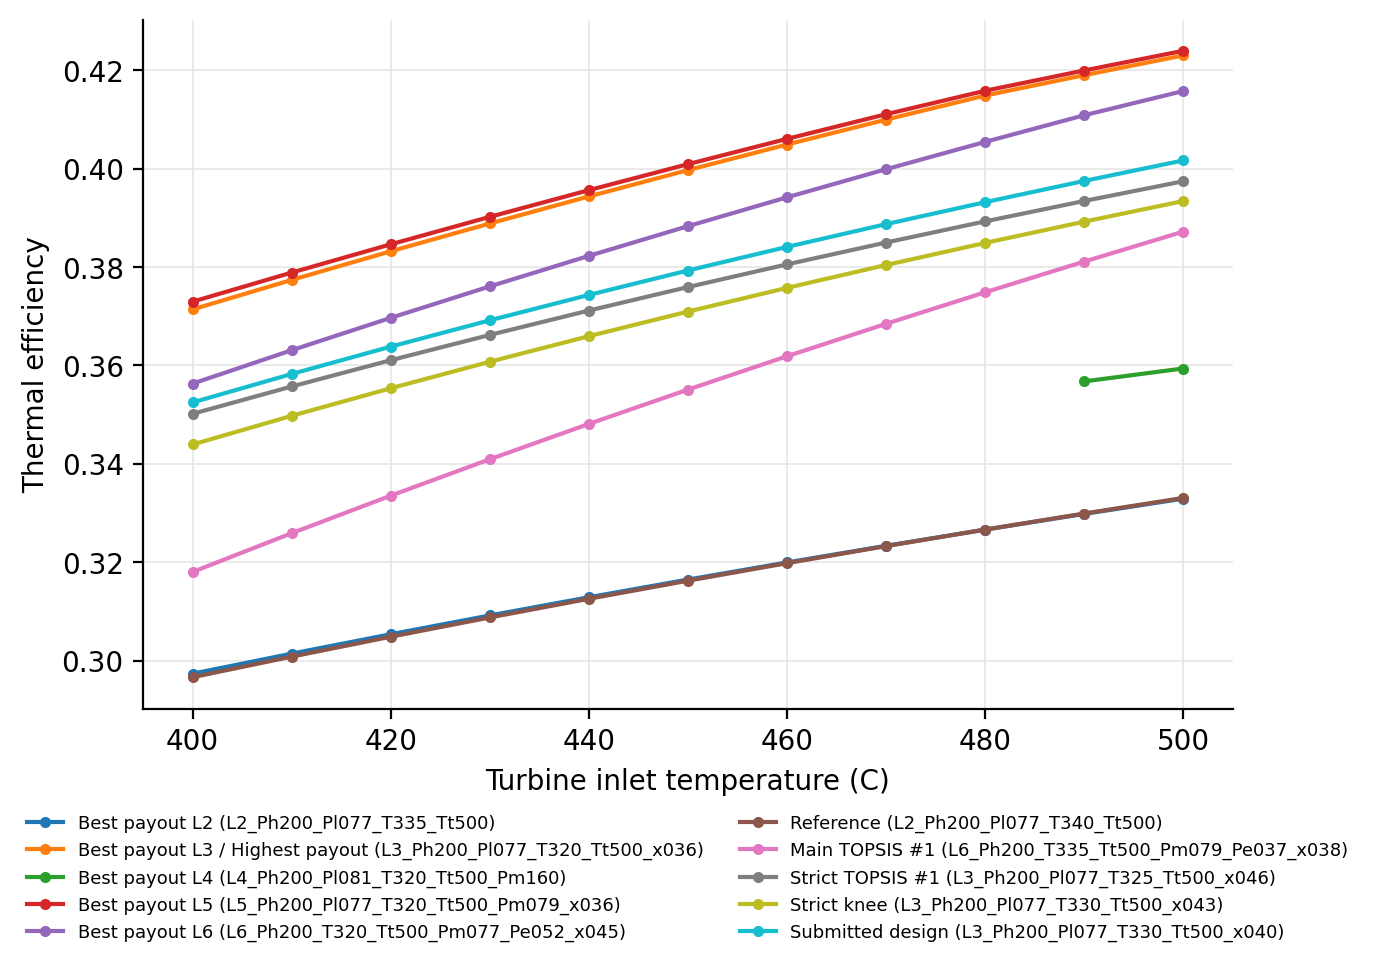
\includegraphics[width=0.8\textwidth]{figs/s6_tturb.png}
\caption{S6: efficiency against turbine inlet temperature, other variables fixed.}\label{fig:s6}
\end{figure}

\paragraph{S7: turbine inlet pressure.} The named designs were re-solved from 14 to \SI{20}{MPa} (Figure~\ref{fig:s7}). Efficiency and payout still rise at \SI{20}{MPa} in every case, so the limit is binding, but the gain is small for the recommended designs: under \$1M per MPa for the selected and strict designs, against \$2.7M per MPa for the recuperated reference.

\begin{figure}[h]\centering
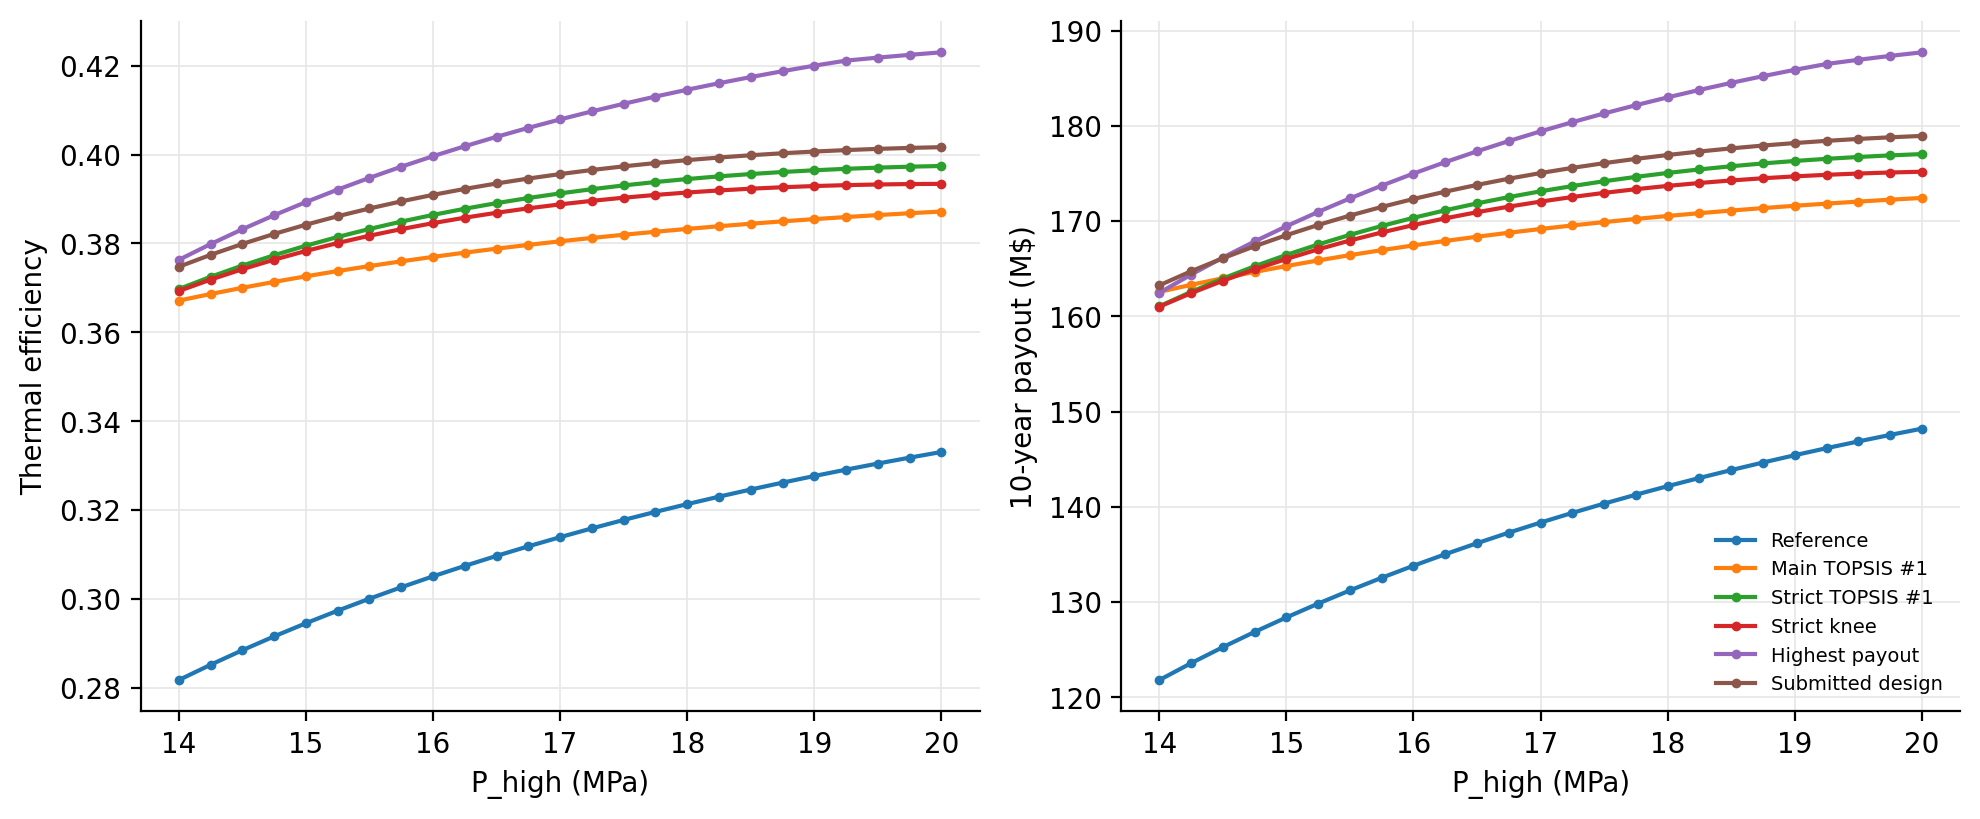
\includegraphics[width=\textwidth]{figs/s7_phigh.png}
\caption{S7: efficiency (left) and payout (right) against turbine inlet pressure for the named designs.}\label{fig:s7}
\end{figure}

\paragraph{S8: the simple cycle with pressurised water.} The nine simple-cycle designs that failed at \SI{6}{bar} were solved by raising the water pressure for layout 1 only. 20 bar recovers 13 of the 18 designs, 50 bar 15, and \SI{100}{bar} all 18. The water pressure changes only the water side. The best simple cycle reaches 14.9\% and \$60.9M, so its exclusion from the ranking is unaffected.

\paragraph{S9: exchanger temperature profiles.} Every exchanger of the named designs was drawn as temperature against duty at 100 slices, with its pinch marked (Figure~\ref{fig:s9}). Every cooler reaches its \SI{5}{K} pinch inside the exchanger, where the \cotwo{} crosses its pseudo-critical region, about a quarter to a third of the duty from the cold end. The exception is the selected design's first cooler, ahead of the pre-compressor, which works on the low-pressure gas and has its pinch at the hot end. All recuperator pinches lie well above \SI{5}{K} (\SI{10.4}{K} and more), which confirms that the \SI{0.90}{} effectiveness, not the pinch limit, sizes the recuperators of these designs.

\begin{figure}[h]\centering
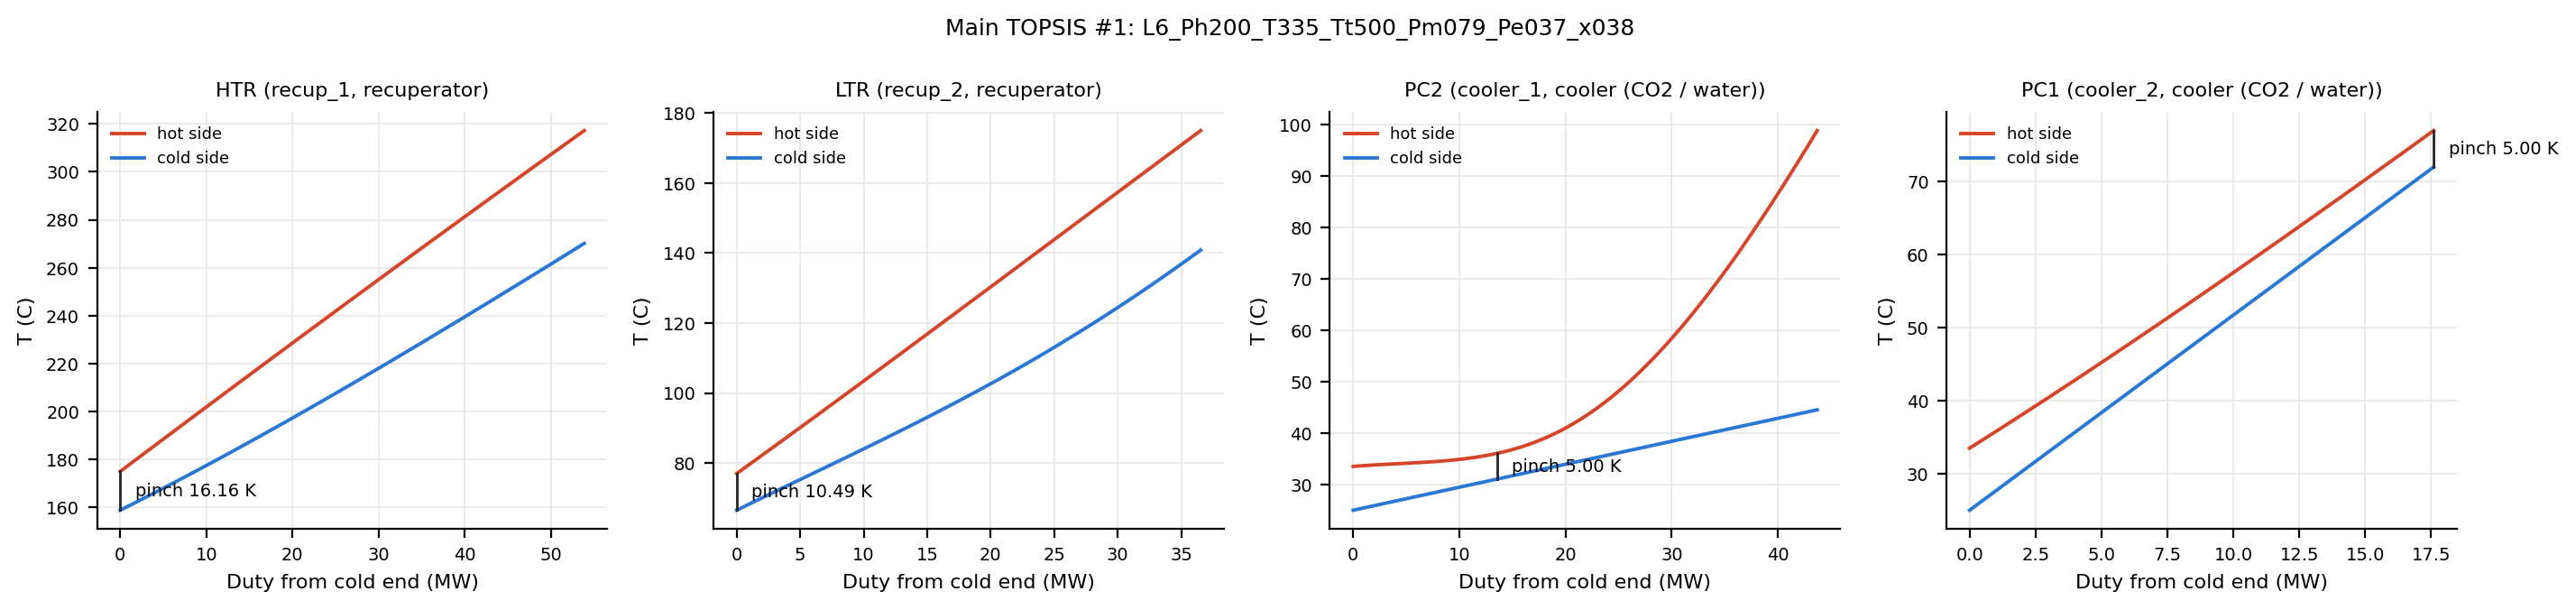
\includegraphics[width=\textwidth]{figs/s9_tq_selected.png}
\caption{S9: temperature against duty for the four exchangers of the selected design, with the pinch of each marked.}\label{fig:s9}
\end{figure}

\paragraph{Overall.} No study overturns the recommendation outright. The selected partial-cooling design holds under pressure drops, discounting, a larger cooler pinch, moderate price differences, and lower turbine temperature or pressure, and in the frozen-hardware test it loses a quarter as much efficiency to inlet temperature drift as the recompression designs. It gives way to recompression in three cases: a \SI{3}{K} cooler pinch, exchangers much cheaper per kilogram than machines, and (for the knee only) a 20-year horizon with little discounting. In each of these the replacement is the strict winner region: recompression at 20 / \SI{7.7}{MPa}, \SI{32.5}{\celsius} and $x \approx 0.44$ to 0.47. The two candidates of Section~\ref{sec:results} therefore remain the two candidates after every test.

\code{\path{core/studies/}, \path{out/studies/}; \path{out/studies/README.md} summarises every study}
